\section{Field of view of a drop in a sphere}
\label{sec:app-geom-drop-fov}

\begin{figure}
	\centering
	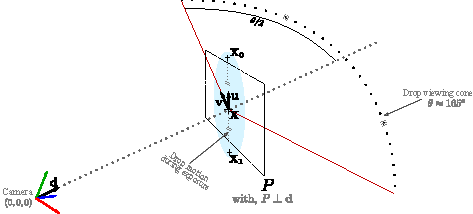
\includegraphics[width=1.0\linewidth]{figures/suppl/drop_fov_geom.pdf}
	\caption{Geometrical construction to compute a drop FOV. Considering $\mathbf{X_0}$ and $\mathbf{X_1}$ the drop position at shutter opening and closing, respectively. We assume a constant drop position $\mathbf{X} = \frac{\mathbf{X_0}+\mathbf{X_1}}{2}$ (during the exposure time, a few milliseconds). Note that we drew only a slice of the drop FOV for simplicity but a full 3D visualization would show a full 3D cone. The drop FOV \textit{in} the environment map is the projection of the 3D drop FOV on the scene sphere of constant distance (refer to text for details).}
	\label{fig:drop_fov_geom}
\end{figure}

We estimate the field of view (FOV) of a drop when projected on a sphere to compute the radiance and chromaticity of each streak, as detailed in sec.~3.3 of the main paper. 
Despite its motion, we make the assumption of a constant field of view within a given exposure time. This is acceptable due to the short exposure time used here (i.e. 2ms for KITTI, 5ms for Cityscapes).
For each drop, the simulator outputs the start position (i.e. shutter opening) and end position (i.e. shutter closing) in both the 3D camera-centered and the 2D image coordinate frames.

We refer to the fig. \ref{fig:drop_fov_geom} for a geometrical illustration of the following.
Let us consider an imaged drop $D$, having 3D start position $\mathbf{X_0}$ and end position $\mathbf{X_1}$. We first compute $\mathbf{X} = \frac{\mathbf{X_0}+\mathbf{X_1}}{2}$ the \textit{assumed constant} position for which we will estimate the corresponding FOV. 
The position being camera-centered, the drop viewing direction is therefore $\mathbf{d}=\frac{\mathbf{X}}{||\mathbf{X}||}$. 

We compute the equation of the plane $P$ going through $\mathbf{X}$ and orthogonal to the viewing direction $\mathbf{d}$:
\begin{equation}
P = \mathbf{d}_x+\mathbf{d}_y+\mathbf{d}_z-\mathbf{d}\cdot\mathbf{X} = 0\,,
\end{equation}
where $\cdot$ is the dot product and select a random vector $\mathbf{u}$ (with $||\mathbf{u}|| = 1$) lying on $P$. 
Accounting for the field of view of the drop $\theta\approx165^\circ$ (according to \cite{garg2007vision}), we compute an arbitrary vector $\mathbf{v}$ on the viewing cone \textit{through} the drop
\begin{equation}
\mathbf{v} = \mathbf{d}\cdot\mathbf{R}_{\mathbf{u}}(\theta/2)\,,
\end{equation}
with $\mathbf{R}_{\mathbf{u}}(\theta/2)$ the 3x3 general rotation matrix of angle $\theta/2$ about vector $\mathbf{u}$. 
We use $\theta/2$ because the cone being symmetric along the viewing direction, the complete cone field of view obtain is $\theta$. 
The set $V'$ of vectors forming the viewing cone through the drop is obtained by the rotation of $\mathbf{v}$ all around the viewing direction. Formally,
\begin{equation}
V' = \{\mathbf{v}\cdot\mathbf{R}_{\mathbf{d}}(\alpha) ~| ~\forall ~\alpha \in [0, 2\pi[\}\,,
\end{equation}
with $\mathbf{R}_{\mathbf{d}}(\alpha)$ the rotation matrix of $\alpha$ around vector $\mathbf{d}$. In practice, $V'$ is a finite set of radially equidistant vectors (for computational reason we use $|V'| = 20$).

To compute the coordinates of the drop FOV in the environment, we assume a projection sphere $S$ of radius $10$m. Hence, we compute the set $Q = \{\phi(S, \mathbf{v'}) ~| ~\forall ~\mathbf{v'} \in V'\}$ of points where vectors intersect the environment sphere, considering only the positive viewing direction axis. 
Given that the sphere is centered to the camera position and all drops 3D positions are expressed in the camera referential, the intersection $\phi(S, \mathbf{v'})$ of a vector $\mathbf{v'}$ and sphere $S$ of radius $S_{\rho}$ is straight-forward with
\begin{equation}
\begin{split}
\phi(S, \mathbf{v'}) &= \mathbf{v'} + t\mathbf{d}\,\text{with},\\
t &= \frac{-b + \sqrt{b^2 - 4ac}}{2a}\,,\\
a &= \mathbf{d}_x^2 + \mathbf{d}_y^2 + \mathbf{d}_z^2\,,\\
b &= 2(\mathbf{d}_x\mathbf{v'}_x + \mathbf{d}_y\mathbf{v'}_y + \mathbf{d}_z\mathbf{v'}_z)\,,\\
c &= \mathbf{v'}_x^2 + \mathbf{v'}_y^2 + \mathbf{v'}_z^2 - S_{\rho}^2\,.
\end{split}
\label{eq:sphere-ray-intersection}
\end{equation}
Having computed $Q$, the finite set of 3D positions intersecting our environment sphere $S$, the set $Q'$ of spherical coordinates (azimuth, altitude) are obtained from simple Cartesian to spherical mapping, and directly translated to the environment map. 
Thus, $Q'$ is the projection of the drop FOV on the environment map.

Accounting for implementation details, one may note that $Q'$ is a discrete representation of the drop field of view contours. In practice, a polygon filling algorithm is used to obtain the drop FOV $F$, which we use for computing the photometry of a rainstreak (cf. sec.~3.3.2 of the main paper).

